\documentclass[11pt, a4paper]{book}
\usepackage{appendix}
\usepackage{amsmath}
\usepackage{amssymb}
\usepackage{cite}
\usepackage{eurosym}
\usepackage{german}
\usepackage[T1]{fontenc}
\usepackage{graphicx}
\usepackage[utf8]{inputenc}
\usepackage{listings}
\usepackage{longtable}
\usepackage{mathptmx}
\usepackage{setspace}
\usepackage{tabularx}
\usepackage{titletoc}
\usepackage{microtype}
\usepackage{pdfpages}
\usepackage[hyphens]{url}
\usepackage[colorlinks=true, linkcolor=blue, citecolor=blue, urlcolor=blue]{hyperref}
\DisableLigatures{}
\pagestyle{headings}
\setcounter{tocdepth}{2}
\setcounter{secnumdepth}{3}

\begin{document}
  \frontmatter
  \pagenumbering{Roman}
  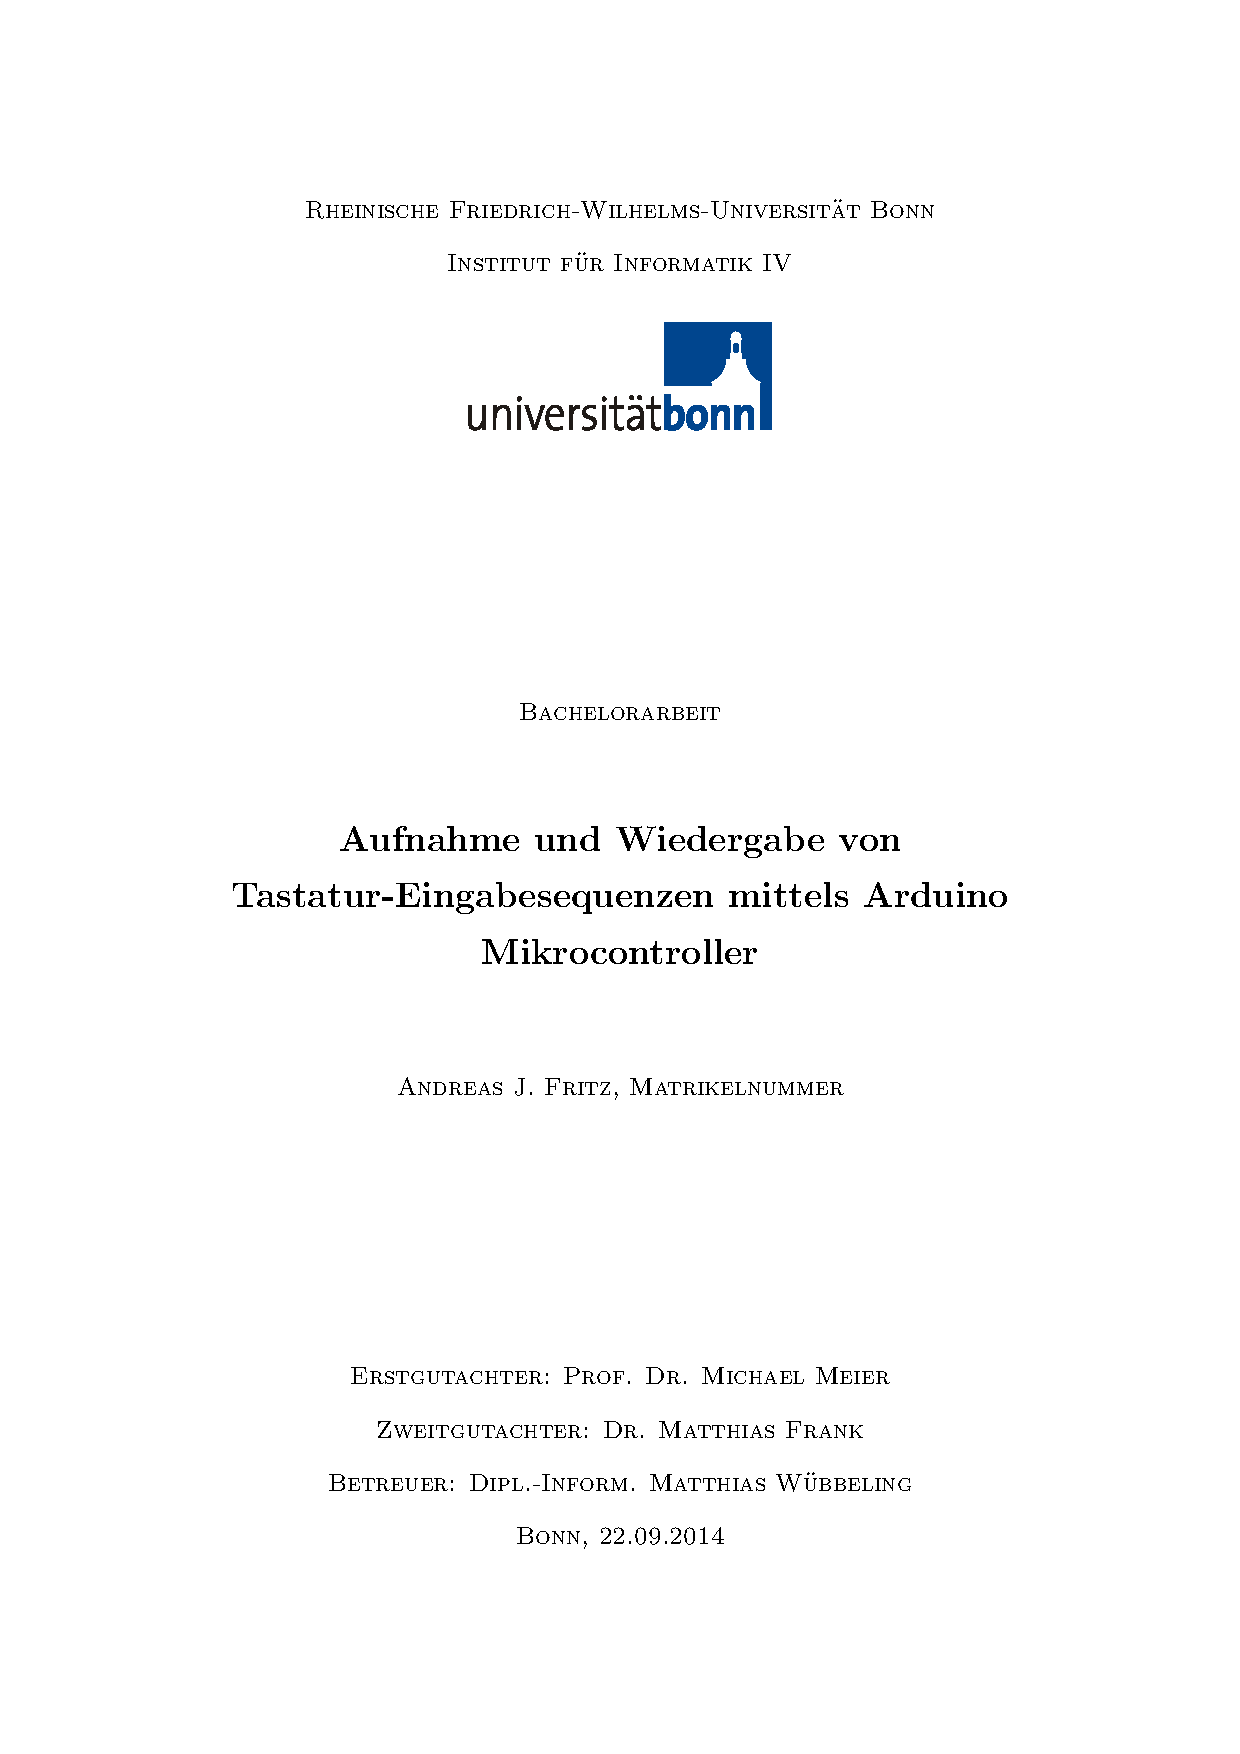
\includepdf{cover}
  \addcontentsline{toc}{chapter}{Zusammenfassung}
\chapter*{Zusammenfassung}
Das Ziel dieser Bachelorarbeit ist es zu zeigen, wie die Aufnahme und Wiedergabe von Tastatur-Eingabesequenzen mittels eines Arduino Mikrocontrollers realisierbar ist. Demonstriert wird dies durch die Implementierung von drei Funktionalitäten, welche die PS/2-Schnittstelle zur Kommunikation verwenden. Dabei handelt es sich erstens um die Aufnahme von Tastatureingaben, zweitens um die Wiedergabe von Tastatureingaben mithilfe einer SD-Karte und drittens um die Wiedergabe von Tastatureingaben über Ethernet. Anschließend werden die genannten Funktionalitäten getestet und darauf hinsichtlich ihrer Korrektheit und Grenzen evaluiert. Schließlich wird in einem Ausblick erläutert, welche weitergehenden Einsatzmöglichkeiten die Implementierung bieten kann.
  \addcontentsline{toc}{chapter}{Selbstständigkeitserklärung}
\chapter*{Selbstständigkeitserklärung}

Hiermit bestätige ich, dass ich die vorliegende Bachelorarbeit selbstständig verfasst und keine anderen als die angegebenen Publikationen, Vorlagen und Hilfsmittel benutzt habe. Alle Teile meiner Arbeit, die dem Wortlaut oder dem Sinn nach anderen Werken (einschließlich Internetquellen) entnommen sind, wurden unter der Angabe Literaturverzeichnis kenntlich gemacht. Diese Arbeit ist weder von mir noch von einer anderen Person bereits in einem anderen Institut vorgelegt worden.
\\
\\
\\
\\
Bonn, 22.09.2014 \hspace{5em} Andreas J. Fritz
  \tableofcontents
  \mainmatter
  \chapter{Einleitung}
Die Verwendung von Geräten zum Erfassen von Tastatur-Eingabesequenzen, sogenannten Keyloggern, ist schon seit Mitte der 1970er Jahre publik \cite{engelberg}. Die New York Times berichtete zu dieser Zeit von einer Spionage durch solche Geräte in US-Botschaften und -Konsulaten in Moskau und St. Petersburg, bei welcher IBM Selectric typewriter angegriffen wurden. Es existieren derzeit sowohl Software- als auch Hardware-Keylogger, jedoch lassen sich diese auch noch einmal in verschiedene Unterkategorien unterteilen. So ist z.B. ein Adapter, welcher zwischen Tastatur und PC steckt, wie in Abbildung \ref{keylogger_ps2} \cite{keylogger_ps2} oder \ref{keylogger_usb} \cite{keylogger_usb} dargestellt, eine mögliche Implementierung eines Hardware-Keyloggers. Diese existieren sowohl für PS/2- als auch USB-Tastaturen und sind im Handel frei erhältlich \cite{keelog}.
\begin{figure}
  \centering
  \begin{minipage}{0.45\textwidth}
    \centering
    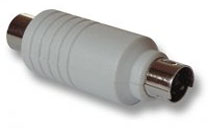
\includegraphics[width=0.6\textwidth]{images/keylogger_ps2.jpg}
    \caption{Keylogger PS/2}
    \label{keylogger_ps2}
  \end{minipage}
  \begin{minipage}{0.45\textwidth}
    \centering
    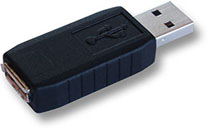
\includegraphics[width=0.6\textwidth]{images/keylogger_usb.jpg}
    \caption{Keylogger USB}
    \label{keylogger_usb}
  \end{minipage}
\end{figure}

Allerdings gelten auch andere Geräte als Hardware-Keylogger, wie z.B. Keypads, welche bei Geldautomaten über das PIN-Feld gelegt werden um den PIN-Code zu erfassen \cite{kirk}. Über Schäden verursacht durch Keylogger existieren allerdings nur wenige Informationen, da Straftaten im Bereich Computerbetrug und Spionage oftmals nicht erkannt oder nicht gemeldet werden \cite{bundeskriminalamt}. So können nur beispielhaft monetäre Erwartungswerte über Schwarzmärkte und spezielle Betrugsdelikte, wie z.B. Kreditkartenbetrug gebildet werden \cite{holz}, oder es werden einzelne Straftaten publik, wie u.a. der versuchte Raub von \$423 Millionen in London \cite{keizer}.

Jedoch ist nicht nur das Mitlesen von Tasteneingaben über die Tastaturschnittstelle möglich, sondern auch die Wiedergabe von Tastatur-Eingabesequenzen, wie u.a. auf der Blackhat Conference demonstriert wurde \cite{chen}. Hierbei wurde die Firmware des Mikrocontrollers derart überschrieben, dass sie nach einer Tasteneingabe und einem zusätzlichen Befehl die Eingabe nochmals in umgekehrter Reihenfolge widergab.

Die vorliegende Bachelorarbeit mit dem Titel ``Aufnahme und Wiedergabe von Tastatur-Eingabesequenzen mittels Arduino Mikrocontroller'' soll jeweils durch eine Implementierung zeigen, dass es einerseits möglich ist Signale einer PS/2-Tastatur mithilfe des Arduino Mikrocontroller \cite{arduino} abfangen und speichern zu können. Andererseits soll gezeigt werden, dass es möglich ist Tastatursignale durch den Mikrocontroller an ein Betriebssystem senden zu können.

Im Folgenden wird sowohl die Idee hinter diesem Thema, als auch mögliche Anwendungen zur Motivation näher beschrieben. Anschließend wird die geplante Herangehensweise für die Bearbeitung dieser Aufgabe geschildert.



\section{Motivation}
Das Aufnehmen und Wiedergeben von Tastatur-Eingabesequenzen bietet viele Möglichkeiten zur Implementierung von nützlichen Funktionalitäten. Im Rahmen dieser Bachelorarbeit dienen drei dieser Funktionalitäten als Motivation und werden dementsprechend mithilfe des Arduino Mikrocontroller \cite{arduino} implementiert:

Die erste Funktionalität ist das einfache Aufzeichnen und Abspeichern der Tastatur-Eingabesequenzen. Dabei sollen die Aufzeichnungen auf einer SD-Karte gespeichert werden, welche beliebig ausgetauscht werden kann.

Als zweite Funktionalität ist das Senden von Tastatursignalen an das Betriebssystem gedacht, welche als Skript auf einer SD-Karte hinterlegt sein können. Nach dem Aufrufen einer Konsole mittels Tastaturkürzeln, die abhängig vom jeweiligen Betriebssystem sind, kann so jeglicher Befehl auf dem System ausgeführt werden. Durch den Einsatz der SD-Karte sind die Skripte austauschbar, sodass verschiedenste Anwendungsmöglichkeiten bestehen.

Die dritte Funktionalität beinhaltet auch das Senden von Tastatursignalen an das Betriebssystem, jedoch werden diese über Ethernet an den Mikrocontroller übertragen. Dies ermöglicht, sofern der Zugriff auf eine Konsole möglich ist, die Steuerung eines Betriebssystems in Echtzeit. Damit gleicht diese Funktionalität einem Remote-Zugriff, jedoch ohne den Einsatz von Software auf dem zu steuernden Betriebssystem.

Da es sich bei den letzten beiden Funktionalitäten um das Senden von Tastatursignalen über das PS/2-Protokoll handelt, besteht weiterhin die Möglichkeit, dass die eingegebenen Befehle ohne eine explizite Prüfung des Betriebssystems oder eines Virenscanners ausgeführt werden können. Dies zu evaluieren ist somit ein weiterer Bestandteil dieser Bachelorarbeit und kann mit Folgen für die IT-Sicherheit verbunden sein.



\section{Aufbau der Arbeit}
Zu Beginn dieser Bachelorarbeit ist im ersten Kapitel die Recherche bezüglich der PS/2-Tastaturschnittstelle und des PS/2-Protokolls für das weitere Vorgehen erforderlich . Zudem werden verwandte Arbeiten aus dem Bereich der Aufnahme und Wiedergabe von Tastatureingabesquenzen beschrieben und die rechtlichen Grundlagen benannt. Im nächsten Kapitel wird die Implementierung der Funktionalitäten dokumentiert. Dies deckt sowohl die notwendigen Softwarekomponenten für den Arduino Mikrocontroller ab, als auch den Aufbau der Elektronik. In dem darauf folgenden Kapitel werden die Ergebnisse der Implementierung evaluiert und bestehende Abwehrmechanismen beschrieben. Abschließend wird in dem letzten Kapitel die Bachelorarbeit zusammengefasst und ein Ausblick für zukünftige Arbeiten gegeben.
  \chapter{Grundlagen}
Um den Mikrocontroller zu implementieren, der Tastatureingabesequenzen sowohl aufnehmen als auch wiedergeben soll, müssen dafür einige Grundlagen benannt werden. Dieses Kapitel beschreibt im Folgenden die benötigten Elemente der PS/2-Tastaturschnittstelle und des PS/2-Protokolls, sowie einige verwandte Arbeiten in dieses Themengebiets als auch die rechtlichen Grundlagen. Die Abschnitte PS/2-Tastaturschnittstelle und PS/2-Protokoll fassen die Beschreibungen von Adam Chapweske \cite{chapweske} bzw. der Übersetzung von Bernward Mock \cite{mock} zusammen.



\section{PS/2-Tastaturschnittstelle}
IBM entwickelte 1987 die PS/2-Tastatur zur Verwendung am gleichnamigen PC, dem Personal System/2, und ist kompatibel mit der zuvor entwickelten AT-Tastatur. Der Anschluss erfolgt über einen 5- oder 6-poligen Mini-DIN Stecker, bzw. alternativ über einen SDL-Stecker. In Abbildung \ref{female_pins} \cite{female_pins} ist die Anordnung der 6 Pins aufseiten des PCs (female) zu sehen. Spiegelverkehrt dazu ist der Anschluss der Tastatur (male).

\begin{figure}
  \centering
  \begin{minipage}{0.45\textwidth}
    \centering
    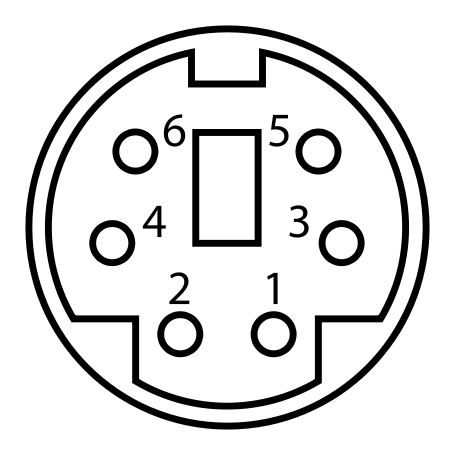
\includegraphics[width=0.48\linewidth]{images/female_pins.png}
    \caption{PS/2 Female Pins}
    \label{female_pins}
  \end{minipage}
  \begin{minipage}{0.45\textwidth}
    \centering
    \begin{tabular}{|l|l|} \hline
      Pin 1 & Daten \\ \hline
      Pin 2 & kein Signal \\ \hline
      Pin 3 & Erdung \\ \hline
      Pin 4 & 5 Volt \\ \hline
      Pin 5 & Takt \\ \hline
      Pin 6 & kein Signal \\ \hline
    \end{tabular}
    \caption{Pin Spezifikation}
    \label{pin_specification}
  \end{minipage}
\end{figure}

Für die Verwendung einer PS/2-Tastatur werden nur 4 der 6 Pins benötigt, da ein Datensignal, eine Erdung, ein Takt und eine Leitung mit 5 Volt ausreichen um Tastensignale zu übertragen (siehe Abbildung \ref{pin_specification}). Ein in der Tastatur verbauter Mikrocontroller, ein sogenannter Keyboard-Encoder, scannt die Tasten und überprüft ob eine Taste gedrückt ist oder nicht. PS/2-Tastaturen verwenden typischerweise zwischen 84 bis 104 Tasten, welche sogenannten Scancodes zugeordnet werden. Es existieren drei Scancode-Sets, wobei PS/2-Tastaturen den als Scancode-Set 2 bekannten Satz benutzen. In Abbildung \ref{scancodes} \cite{scancodes} ist ein Ausschnitt dieser Scancodes auf einigen Tasten zu sehen und im Anhang befindet sich die Tabelle \ref{scancode_set_2} des gesamten Scancode-Sets 2.

\begin{figure}
  \centering
  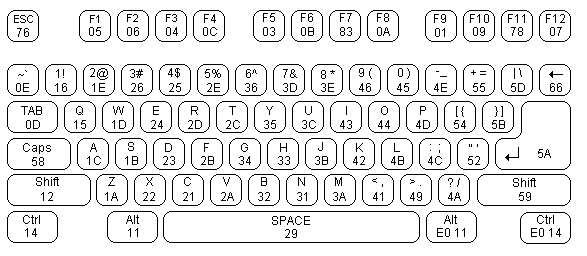
\includegraphics[width=0.9\textwidth]{images/scancodes.jpg}
  \caption{Scancode-Set 2 Ausschnitt}
  \label{scancodes}
\end{figure}

Die Scancodes sind Hexadezimalwerte bestehend aus einem Makecode, welcher gesendet wird wenn die Taste gedrückt wird, und einem Breakcode, der beim Loslassen der Taste gesendet wird. Breakcodes setzen sich in fast allen Fällen aus einem 0xf0 und dem Makecode der Taste zusammen. Zudem existieren erweiterete Tasten, deren Makecode länger als ein Byte ist und zusätzlich ein 0xe0 als erstes Byte haben, was auch für den zugehörigen Breakcode gilt. Um also z.B. ein ``G'' wiederzugeben ist es notwendig zuerst die Shift-Taste gedrückt zu halten, die G-Taste zu drücken und beide Tasten in umgekehrter Reihenfolge loszulassen. Dementsprechend können für dieses Beispiel die folgenden Scancodes übertragen werden: 0x12 (Make L Shift), 0x34 (Make G), 0xf0 0x34 (Break G) und 0xf0 0x12 (Break L Shift).

Wenn eine Taste dauerhaft gedrückt wird setzt die Wiederholfunktion des Mikrocontrollers der Tastatur ein, auch Typematic genannt. Diese sendet mit einer gewissen Verzögerung (typematic delay) den Makecode der zuletzt gedrückten Taste und dann mit einer bestimmten Wiederholrate (typematic rate) fortwährend denselben Makecode, bis die Taste losgelassen wird. Beide Parameter können durch den PC, in diesem Zusammenhang auch Host genannt, eingestellt werden, wobei die Verzögerung zwischen 0,25 und 1,00 Sekunden liegen kann und die Wiederholrate zwischen 2,0 cps und 30,0 cps (Zeichen pro Sekunde).

Die Tastatur kann weiterhin einen Reset vollziehen und führt dabei einen Selbsttest, auch Basic Assurance Test (BAT) genannt, durch. Dabei wird die Verzögerung auf 0,5 Sekunden und die Wiederholrate auf 10,9 cps gesetzt, sowie Scancode-Set 2 geladen. Zudem werden zu Beginn des BAT die drei LEDs der Tastatur an und danach wieder ausgeschaltet, sowie 0xaa an den Host gesendet für ein erfolgreich abgeschlossenen BAT.

Die Kommunikation zwischen dem Host und der Tastatur wird im folgenden Abschnitt anhand des PS/2-Protokolls beschrieben.



\section{PS/2-Protokoll}
Bei dem PS/2-Protokoll handelt es sich um ein sogenanntes bi-direktionales serielles Protokoll. Dies bedeutet, dass auch der Host Befehle an die Tastatur senden kann, im Fall des PS/2-Protokolls sind es 17 Host-Befehle. Eine detaillierte Auflistung dieser Befehle zeigt die Tabelle ... im Anhang.
\begin{figure}
  \centering
  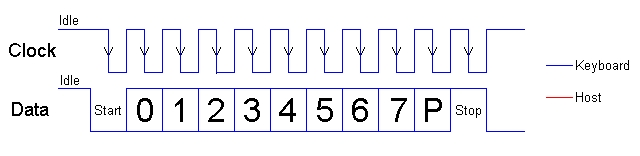
\includegraphics[width=1\textwidth]{images/device_to_host.jpg}
  \caption{Kommunikation Tastatur zu Host}
  \label{device_to_host}
\end{figure}
1 Startbit, immer 0
8 Datenbits mit LSB voran
1 Parity-Bit (ungerade Parität)
1 Stopbit, immer 1
ggf. 1 ACK-Bit (nur bei Host zu Tastatur)



\section{Verwandte Arbeiten}
Wie bereits in der Einleitung erwähnt, existieren viele Produkte im Bereich der Hardware-Keylogger. So gibt es bereits Keylogger für USB-Tastaturen und PS/2-Tastaturen mit verschiedenen Speichergrößen oder der Möglichkeit die aufgezeichneten Tastatureingaben über Wi-Fi zu versenden \cite{keelog}.

Im Bereich der Mikrocontroller gibt es verschiedene Bibliotheken, die das Mitlesen von Tastatureingaben ermöglichen. Eine verbreitete Implementierung ist eine Bibliothek, die sowohl für Arduino Mikrocontroller als auch andere Mikrocontroller gedacht ist \cite{ps2keyboard}. Die bereitgestellten Funktionen erlauben es, wie in den mitgelieferten Beispielen gezeigt wird, die Tastatureingaben der mit dem Mikrocontroller verbundenen Tastatur über den Mikrocontroller auszugeben. Auch in anderen Implementierungen, wie z.B. dem Tastaturtreiber des Betriebssystems PrettyOS, werden Tastatureingaben entgegen genommen und in ASCII-Zeichen umgewandelt, um diese u.a. auf dem Bildschirm auszugeben \cite{prettyos}.

Es wurden aber auch Konzepte und deren Umsetzung dokumentiert, welche die Manipulation von Tastatureingaben zeigen. In einem bestehenden Ansatz wurde die Firmware des Mikrocontrollers einer Apple-Tastatur überschrieben \cite{chen}. Dies hatte zur Folge, dass nach einer normalen Zeicheneingabe und einer bestimmten Befehlsequenz diese Zeicheneingabe erneut, aber spiegelverkehrt an den PC gesendet wurde.

Andere Ansätze werden zudem als Produkt vertrieben, wie z.B. der USB-Stick Rubber Ducky \cite{ducky}. Dieser enthält unter seiner Abdeckung einen zusätzlichen Mikrocontroller mit einer Speicherkarte. Mithilfe von eigenen Befehlen, die in einer Textdatei auf der Speicherkarte gespeichert werden kann, führt der USB-Stick diese Befehle als Tastatureingaben aus, sobald er mit einem PC verbunden wird.

Zuletzt wurde ein weiterer Ansatz präsentiert, welcher BadUSB \cite{badusb},

Der Unterschied zu dem Ansatz dieser Bachelorarbeit besteht darin, dass für die Wiedergabe von Tastatureingabesequenzen nicht der Mikrocontroller der Tastatur angepasst werden soll. Stattdessen wird ein eigener Mikroccontroller die Tastatureingaben tätigen, die vorher dem Mikrocontroller entweder via SD-Karte oder Ethernet übergeben wurden.



\section{Rechtliche Grundlagen}
Die rechtlichen Grundlagen für den Einsatz technischer Hilfsmittel zum unbefugten Aufzeichnen oder Manipulieren von Daten sind differenziert zu betrachten, denn meist ist die Rechtmäßigkeit einer Verwendung fallbezogen. Der Paragraph \S 202a Strafgesetzbuch \cite{stgb} regelt den unbefugten Zugriff auf Daten folgendermaßen:
\begin{quote}
  (1) Wer unbefugt sich oder einem anderen Zugang zu Daten, die nicht für ihn bestimmt und die gegen unberechtigten Zugang besonders gesichert sind, unter Überwindung der Zugangssicherung verschafft, wird mit Freiheitsstrafe bis zu drei Jahren oder mit Geldstrafe bestraft. \\
  (2) Daten im Sinne des Absatzes 1 sind nur solche, die elektronisch, magnetisch oder sonst nicht unmittelbar wahrnehmbar gespeichert sind oder übermittelt werden.
\end{quote}
Dies bedeutet zum Bespiel, dass es verboten ist mithilfe eines Hardware-Keyloggers die Tastatureingaben einer anderen Person unbefugt aufzuzeichnen.

Auch einem Arbeitgeber ist es im Allgemeinen nicht gestattet, Daten der Arbeitnehmer ohne deren Wissen festzuhalten \cite{bildscharbv}. Darüber hinaus regelt das Betriebsverfassungsgesetz, dass der Betriebsrat bei der Einführung technischer Hilfsmittel zur Aufzeichnung von Verhalten und Leistung der Arbeitnehmer Mitbestimmungsrechte besitzt \cite{betrvg}.

Anders verhält es sich beim Einsatz technischer Hilfsmittel zum Aufzeichnen von Daten bzgl. der Strafverfolgung. Zwar ist \S 100h Abs. 1 Nr. 2 Strafprozessordnung \cite{stpo} laut einer internen Einschätzung der Generalstaatsanwaltschaft München \cite{munich} nicht ausreichend, jedoch wurde mit \S 20k BKA-Gesetz \cite{bkag} entsprechende Grundlagen für den Einsatz solcher Hilfsmittel geschaffen. Somit ist z.B. der Einsatz von ``Remote Forensic Software'' (ugs. ``Bundestrojaner'') unter bestimmten Umständen möglich, welcher eine Funktion zur Aufzeichnung von Tastatureingaben besitzt \cite{spd}.
  \chapter{Implementierung}
Die Umsetzung der zu Beginn beschriebenen Funktionalitäten wird innerhalb der folgenden Teilabschnitte beschrieben. Der erste Teilabschnitt dieses Kapitels dokumentiert die entwickelte Software \cite{badps2}, welche den Mikrocontroller steuert und den Programmablauf der einzelnen Funktionalitäten zeigt. Der zweite Teil dieses Kapitels erläutert den Aufbau der Elektronik und zeigt wie die verwendete Hardware mit dem Mikrocontroller zusammengebaut wurde.



\section{Softwaredokumentation}
Die implementierten Softwarekomponenten \cite{badps2} gliedern sich in die drei  Diese beinhalten Hilfsfunktionen für die Tastatur, für die SD-Karte und für die Webseite, welche vorab in den nächsten Abschnitten beschrieben werden.

\subsection{Hilfsfunktionen für die Tastatur}
\subsubsection{void initKeys(int dataPin, int clockPin)}
\subsubsection{void setHigh(int pin)}
\subsubsection{void setLow(int pin)}
\subsubsection{unsigned char readKeys(int dataPin, int clockPin)}
\subsubsection{void sendKeys(int dataPin, int clockPin, unsigned char data)}
\subsubsection{void writeKeys(unsigned char data)}


\subsection{Hilfsfunktionen für die SD-Karte}
\subsubsection{void initCard(int sdPin)}
\subsubsection{String readFile(char* filename)}
\subsubsection{void writeFile(char* filename, String content)}
\subsubsection{void deleteFile(char* filename)}


\subsection{Hilfsfunktionen für die Webseite}
\subsubsection{void sendWebsite(EthernetClient client, String serverState)}


\subsection{Aufnahme von Tastatureingaben}
\begin{figure}
  \centering
  %\includegraphics[angle=90,width=1\textwidth]{images/diagram_reader.png}
  \caption{Aktivitätsdiagramm für die Methode reader()}
  \label{diagram_reader}
\end{figure}


\subsection{Wiedergabe von Tastatureingaben mittels SD-Karte}
\begin{figure}
  \centering
  %\includegraphics[angle=90,width=1\textwidth]{images/diagram_writer.png}
  \caption{Aktivitätsdiagramm für die Methode writer()}
  \label{diagram_writer}
\end{figure}


\subsection{Wiedergabe von Tastatureingaben über Ethernet}
\begin{figure}
  \centering
  %\includegraphics[angle=90,width=1\textwidth]{images/diagram_sender.png}
  \caption{Aktivitätsdiagramm für die Methode sender()}
  \label{diagram_sender}
\end{figure}


\subsection{Gesamter Programmablauf}



\section{Aufbau der Elektronik}
Verwendete Kabel \cite{ps2male} \cite{ps2female}, Arduino Mega und Ethernet \cite{arduino} und PS/2-Tastatur.
\begin{figure}
  \centering
  \begin{minipage}{0.45\textwidth}
    \centering
    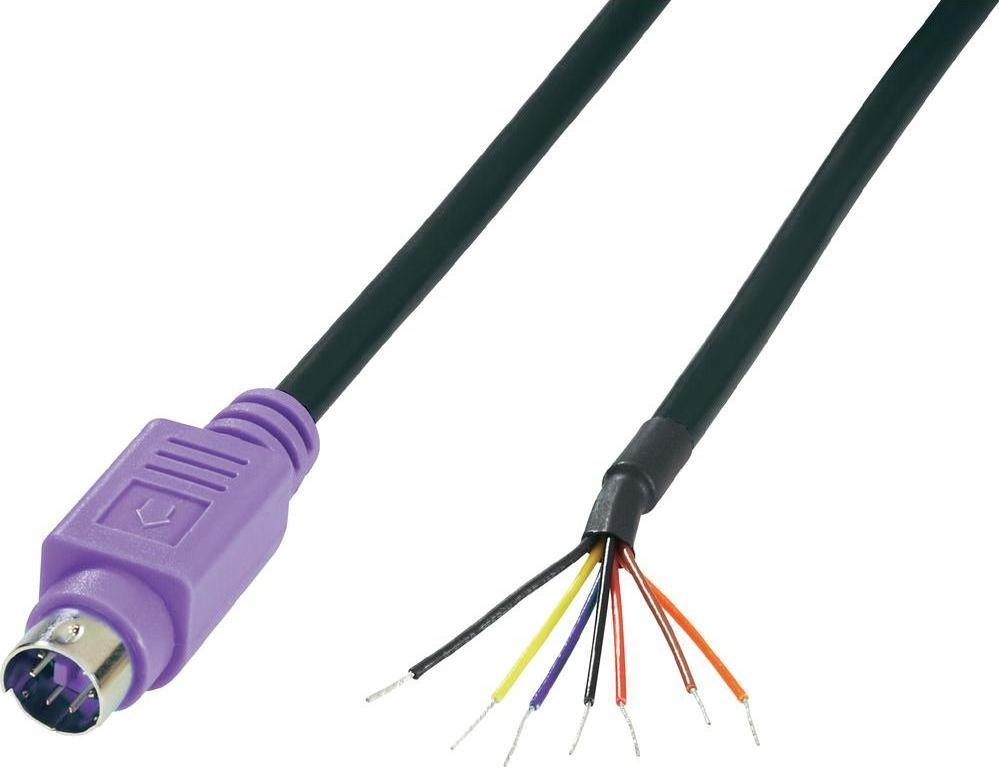
\includegraphics[width=1\textwidth]{images/ps2_male.jpg}
    \caption{PS/2 Male}
    \label{ps2_male}
  \end{minipage}
  \begin{minipage}{0.45\textwidth}
    \centering
    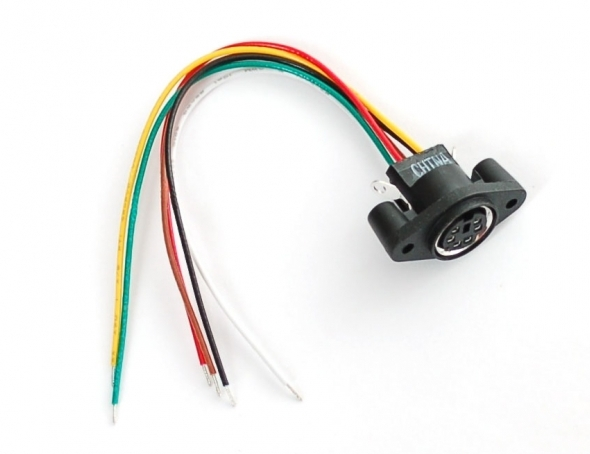
\includegraphics[width=1\textwidth]{images/ps2_female.jpg}
    \caption{PS/2 Female}
    \label{ps2_female}
  \end{minipage}
\end{figure}

\begin{figure}
  \centering
  %\includegraphics[width=0.8\textwidth]{images/hall_effect_sensor.jpg}
  \caption{Schema des Aufbaus fritzing}
  \label{fritzing}
\end{figure}

\begin{figure}
  \centering
  %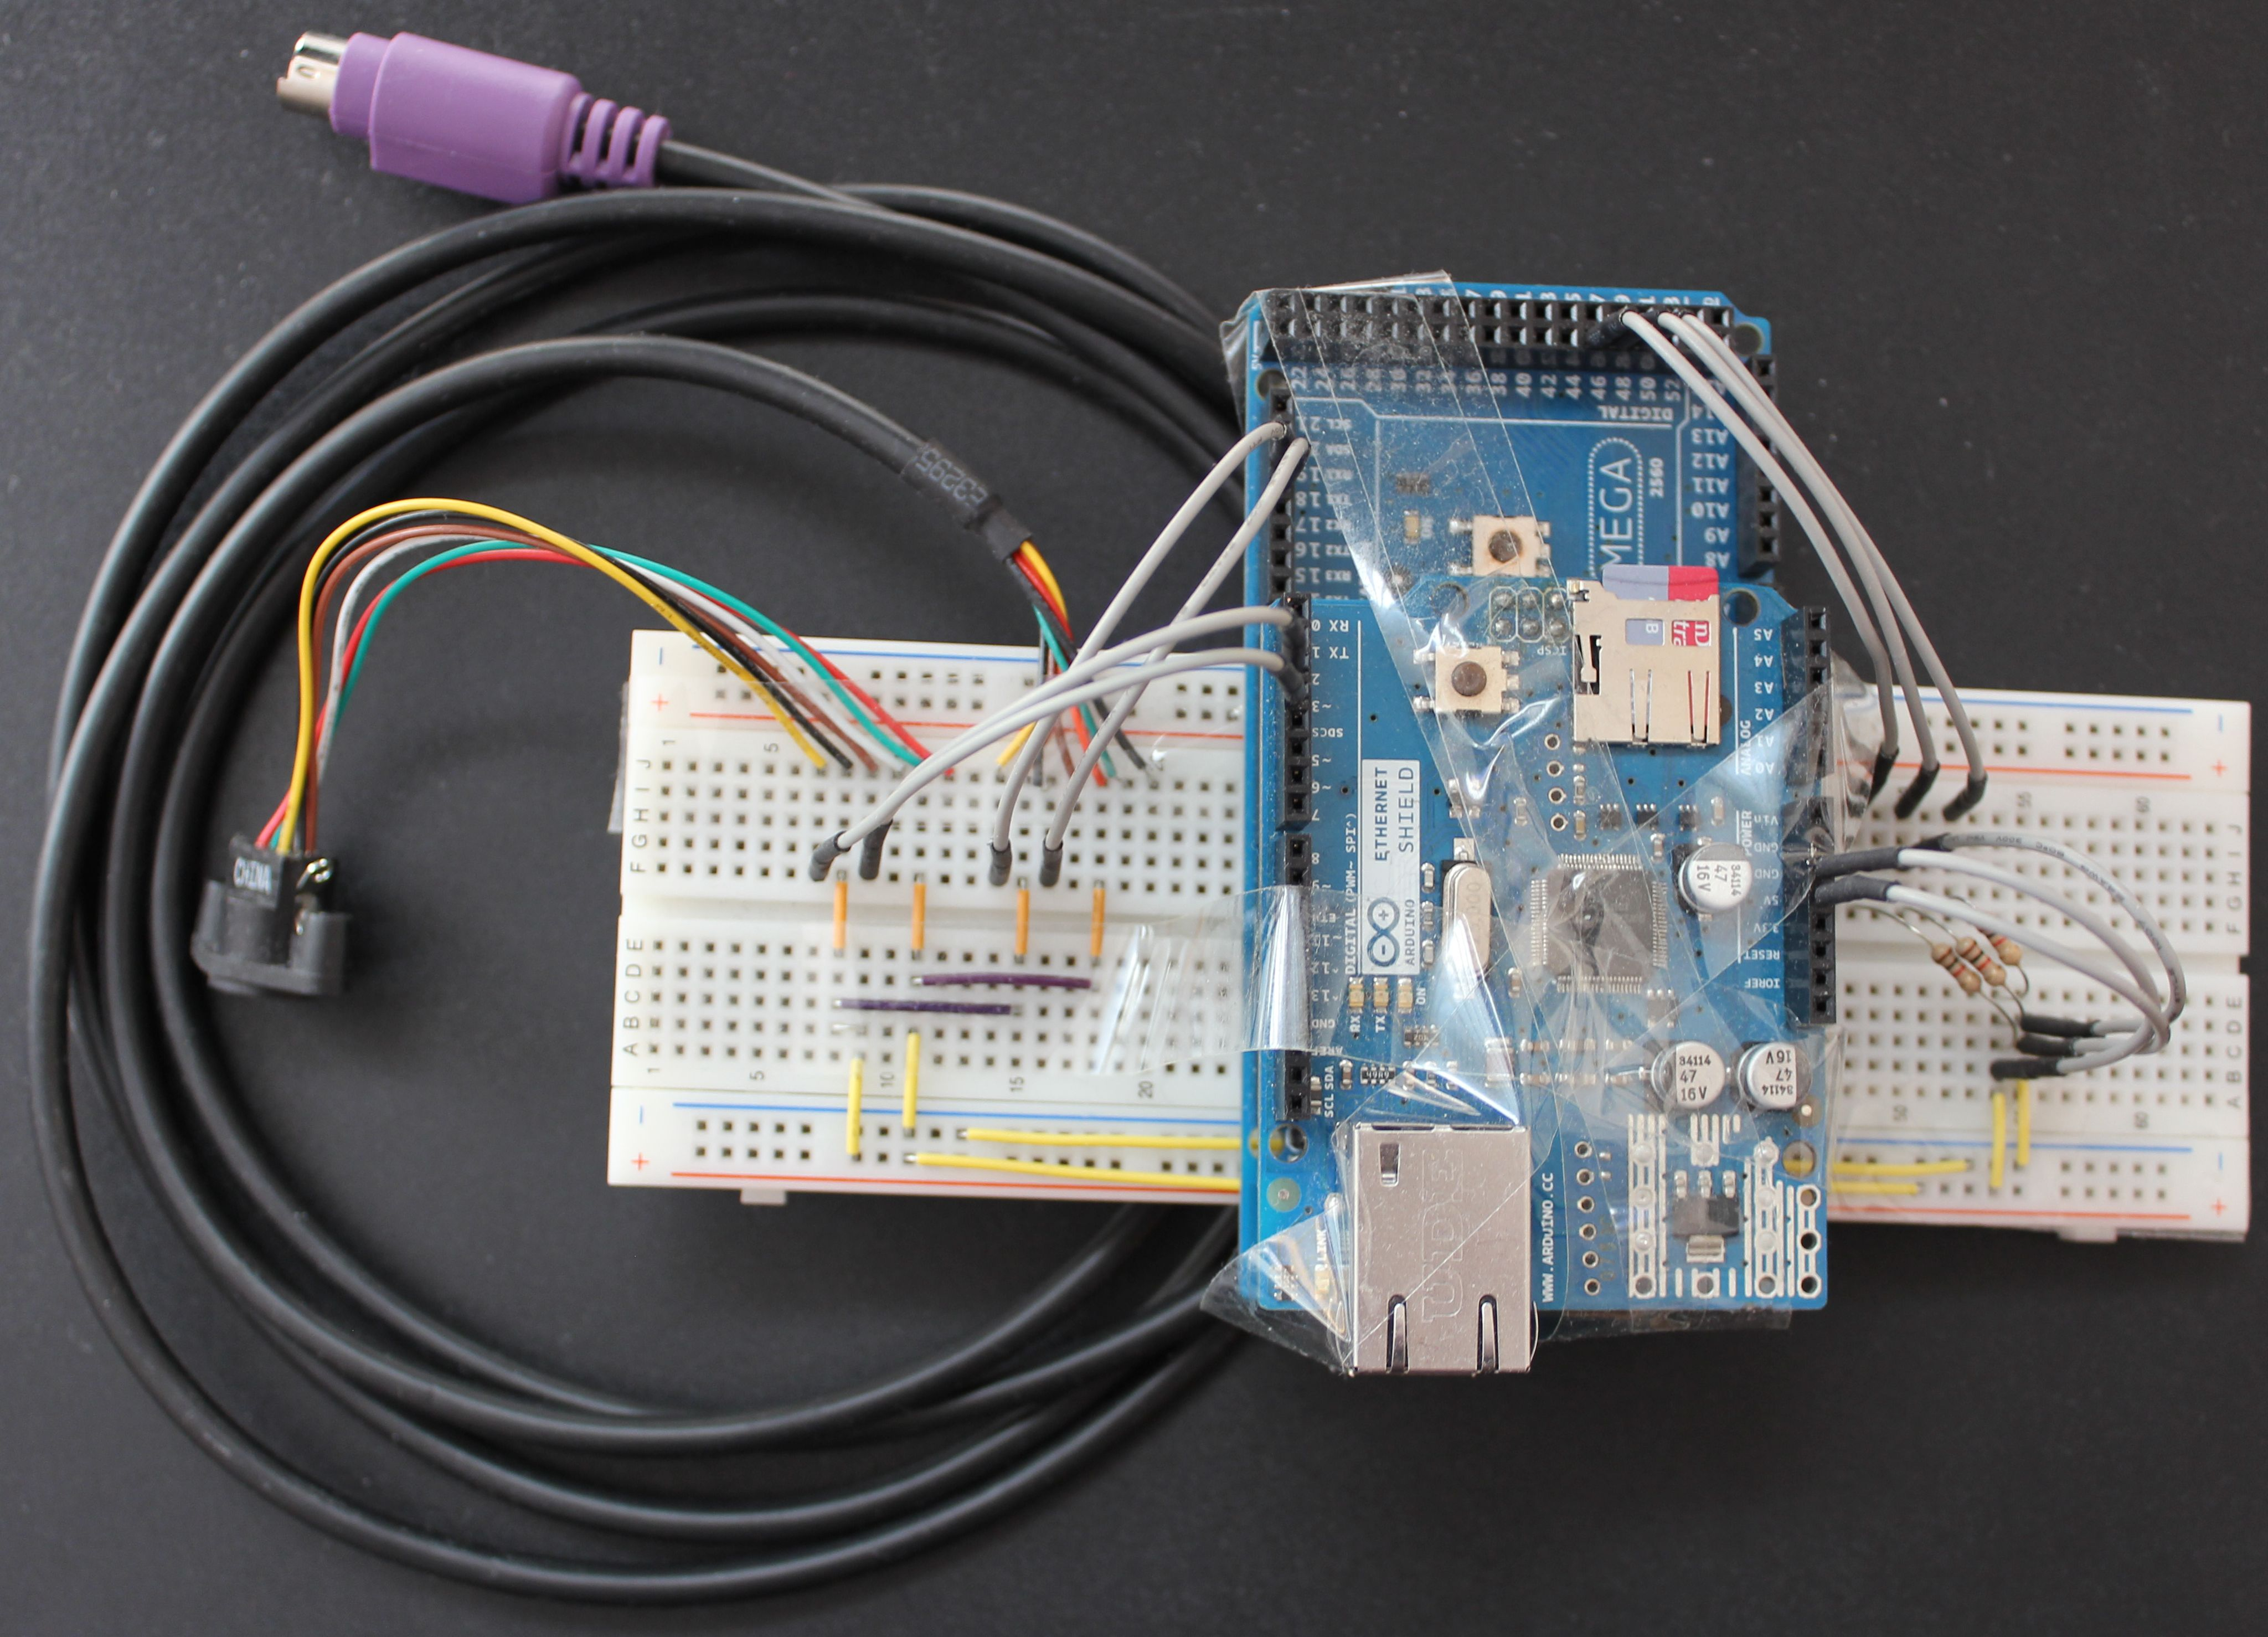
\includegraphics[width=0.8\textwidth]{images/foto1.jpg}
  \caption{Foto des Arduino Ethernet Shields und des Mega 2560 Boards}
  \label{foto1}
\end{figure}
  \chapter{Evaluation}
Test der 3 Funktionalitäten
Für Wiedergabe Test mit Windows und Linux zum Aufruf der Konsole
CTRL ALT T (wait)
xdg-open http://www.google.de ENTER
WINDOWS R (wait) CMD (wait) ENTER
start http://www.google.de ENTER


\section{Abwehrmechanismen}
Mit Host Befehlen testen, wie das Gerät reagiert \cite{mihailowitsch}
  \chapter{Zusammenfassung}
\label{zusammenfassung}
Diese Bachelorarbeit hat dargelegt, wie die Aufnahme und Wiedergabe von Tastatur-Eingabesequenzen mittels Arduino Mikrocontroller über den PS/2-Anschluss realisierbar ist. Zu Beginn der Arbeit wurden in Kapitel \ref{einleitung} drei Funktionalitäten festgelegt, welche im Verlauf der Arbeit implementiert werden sollten, um diese Machbarkeit zu zeigen. Dabei handelte es sich um die Aufnahme von Tastatureingaben, die Wiedergabe von Tastatureingaben mittels SD-Karte und über Ethernet. Anschließend wurden die benötigten Grundlagen im Hinblick auf die spätere Implementierung durch Kapitel \ref{grundlagen} beschrieben. Dazu wurden zuerst die PS/2-Tastaturschnittstelle und das PS/2-Protokoll erläutert, sowie verwandte Arbeiten, Arduino Produkte und rechtliche Grundlagen den Kontext der Arbeit betreffend.

Das darauf folgende Kapitel \ref{implementierung} zeigte die genaue Implementierung der drei Funktionalitäten, sowohl durch die Dokumentation der Software, als auch durch die Beschreibung der Elektronik. Hierbei wurde herausgestellt, wie durch die gezielte Kommunikation über das PS/2-Protokoll mit der Tastatur und dem Host, Signale vom Mikrocontroller entgegengenommen und gesendet werden konnten. Außerdem wurden Methoden zur Interaktion mit der SD-Karte und dem Ethernet-Anschluss dazu verwendet die Funktionalitäten auszubauen. Dabei war es auch nötig die PS/2-Kabel offen mit den Drähten am Steckbrett anzuschließen.

Abschließend griff die Evaluation in Kapitel \ref{evaluation} diese drei Funktionalitäten auf und stellte durch beispielhafte Tastatureingaben die Korrektheit der Implementierung dar, aber auch die bisherigen Grenzen eben dieser Implementierung. Diese äußerten sich u.a. in Beschränkungen bei der Übertragung von der Webseite oder einer fehlenden Rückmeldung an die drei LEDs der Tastatur, falls eine der entsprechenden Tasten gedrückt wurde.

Durch diese Arbeit konnte gezeigt werden, dass sich eine Aufnahme, aber auch eine automatisierte Wiedergabe von Tasteneingaben ggf. auch über Ethernet realisieren lässt. Eingeordnet in den einleitenden Kontext dieser Arbeit bedeutet dies, dass sobald ein physischer Zugang zu einem PC mit PS/2-Anschluss besteht, dieser mithilfe der implementierten Apparatur bedient werden kann. Der folgende Abschnitt gibt einen Ausblick über die sicherheitskritische Relevanz dieser Möglichkeiten.



\section{Ausblick}
Im Zusammenhang dieser Bachelorarbeit wurden die eingangs beschriebenen Funktionalitäten entsprechend implementiert. Im Anschluss daran existieren einige Möglichkeiten die bestehende Arbeit in diesem Bereich fortzuführen. Einerseits können die in der Evaluation beschriebenen Grenzen dieser Implementierung bearbeitet werden, wie z.B. die Übertragungsgröße der Tastatureingaben über die Webseite.

Andererseits wäre der Aspekt der IT-Sicherheit mit möglichen Abwehrmechanismen gegenüber der in dieser Arbeit implementierten Funktionalitäten erwähnenswert. Wie durch die Implementierung gezeigt wurde, ist es möglich über die Wiedergabe von Tasteneingaben die Konsole eines Betriebssystems anzusprechen. Das Erkennen einer automatischen Eingabe könnte dementsprechend eine weitere Option der Fortführung dieser Arbeit sein \cite{mihailowitsch}. Die Ermittlung, ob eine Tastatureingabe von einem Benutzer oder einem Gerät erfolgt, könnte demnach zur Sicherheit eines PCs beitragen.

Schließlich stellt die Manipulation von Tastatur-Eingabesequenzen ein weiteres Feld möglicher Anschlussprojekte dar. Aufbauend auf die Implementierung dieser Bachelorarbeit lassen sich somit spezifsche Tasten oder Tastenkombinationen einer Tastatur sperren oder bestimmte Tasten mit Funktionen belegen. So ließe sich z.B. ein Hardware-Passwortmanager realisieren, der mit dem PS/2-Anschluss und einer entsprechenden Verschlüsselung Anwendung finden könnte.
  \listoffigures
  \addcontentsline{toc}{chapter}{Abbildungsverzeichnis}
  \bibliography{references}{}
  \bibliographystyle{plain}
  \addcontentsline{toc}{chapter}{\bibname}
  \appendix
  \chapter{Anhang}
\section{PS/2-Tastatur Scancode-Set 2}
Die folgenden Angaben sind Hexadezimalwerte für Tastaturen mit 101-, 102- oder 104-Tasten:
\begin{longtable}{| p{.15\textwidth} | p{.14\textwidth} | p{.13\textwidth} || p{.15\textwidth} | p{.14\textwidth} | p{.13\textwidth} |}
  \hline
  \textbf{KEY} & \textbf{MAKE} & \textbf{BREAK} & \textbf{KEY} & \textbf{MAKE} & \textbf{BREAK} \\ \hline
  A & 1c & f0 1c & APPS & e0 2f & e0 f0 2f \\ \hline
  B & 32 & f0 32 & ENTER & 5a & f0 5a \\ \hline
  C & 21 & f0 21 & ESC & 76 & f0 76 \\ \hline
  D & 23 & f0 23 & F1 & 05 & f0 05 \\ \hline
  E & 24 & f0 24 & F2 & 06 & f0 06 \\ \hline
  F & 2b & f0 2b & F3 & 04 & f0 04 \\ \hline
  G & 34 & f0 34 & F4 & 0c & f0 0c \\ \hline
  H & 33 & f0 33 & F5 & 03 & f0 03 \\ \hline
  I & 43 & f0 43 & F6 & 0b & f0 0b \\ \hline
  J & 3b & f0 3b & F7 & 83 & f0 83 \\ \hline
  K & 42 & f0 42 & F8 & 0a & f0 0a \\ \hline
  L & 4b & f0 4b & F9 & 01 & f0 01 \\ \hline
  M & 3a & f0 3a & F10 & 09 & f0 09 \\ \hline
  N & 31 & f0 31 & F11 & 78 & f0 78 \\ \hline
  O & 44 & f0 44 & F12 & 07 & f0 07 \\ \hline
  P & 4d & f0 4d & PRNT SCRN & e0 12 e0 7c & e0 f0 7c e0 f0 12 \\ \hline
  Q & 15 & f0 15 & SCROLL & 7e & f0 7e \\ \hline
  R & 2d & f0 2d & PAUSE & e1 14 77 e1 f0 14 f0 77 & -none- \\ \hline
  S & 1b & f0 1b & [ & 54 & f0 54 \\ \hline
  T & 2c & f0 2c & INSERT & e0 70 & e0 f0 70 \\ \hline
  U & 3c & f0 3c & HOME & e0 6c & e0 f0 6c \\ \hline
  V & 2a & f0 2a & PG UP & e0 7d & e0 f0 7d \\ \hline
  W & 1d & f0 1d & DELETE & e0 71 & e0 f0 71 \\ \hline
  X & 22 & f0 22 & END & e0 69 & e0 f0 69 \\ \hline
  Y & 35 & f0 35 & PG DN & e0 7a & e0 f0 7a \\ \hline
  Z & 1a & f0 1a & U ARROW & e0 75 & e0 f0 75 \\ \hline
  0 & 45 & f0 45 & L ARROW & e0 6b & e0 f0 6b \\ \hline
  1 & 16 & f0 16 & D ARROW & e0 72 & e0 f0 72 \\ \hline
  2 & 1e & f0 1e & R ARROW & e0 74 & e0 f0 74 \\ \hline
  3 & 26 & f0 26 & NUM & 77 & f0 77 \\ \hline
  4 & 25 & f0 25 & KP / & e0 4a & e0 f0 4a \\ \hline
  5 & 2e & f0 2e & KP * & 7c & f0 7c \\ \hline
  6 & 36 & f0 36 & KP - & 7b & f0 7b \\ \hline
  7 & 3d & f0 3d & KP + & 79 & f0 79 \\ \hline
  8 & 3e & f0 3e & KP EN & e0 5a & e0 f0 5a \\ \hline
  9 & 46 & f0 46 & KP . & 71 & f0 71 \\ \hline
  ‘ & 0e & f0 0e & KP 0 & 70 & f0 70 \\ \hline
  - & 4e & f0 4e & KP 1 & 69 & f0 69 \\ \hline
  = & 55 & f0 55 & KP 2 & 72 & f0 72 \\ \hline
  \textbackslash & 5d & f0 5d & KP 3 & 7a & f0 7a \\ \hline
  BKSP & 66 & f0 66 & KP 4 & 6b & f0 6b \\ \hline
  SPACE & 29 & f0 29 & KP 5 & 73 & f0 73 \\ \hline
  TAB & 0d & f0 0d & KP 6 & 74 & f0 74 \\ \hline
  CAPS & 58 & f0 58 & KP 7 & 6c & f0 6c \\ \hline
  L SHFT & 12 & f0 12 & KP 8 & 75 & f0 75 \\ \hline
  L CTRL & 14 & f0 14 & KP 9 & 7d & f0 7d \\ \hline
  L GUI & e0 1f & e0 f0 1f & ] & 5b & f0 5b \\ \hline
  L ALT & 11 & f0 11 & ; & 4c & f0 4c \\ \hline
  R SHFT & 59 & f0 59 & ’ & 52 & f0 52 \\ \hline
  R CTRL & e0 14 & e0 f0 14 & , & 41 & f0 41 \\ \hline
  R GUI & e0 27 & e0 f0 27 & . & 49 & f0 49 \\ \hline
  R ALT & e0 11 & e0 f0 11 & / & 4a & f0 4a \\
  \hline
  \label{scancode_set_2}
\end{longtable}


\section{Befehlssatz}


\section{Quellcode}
\subsection{Microcontroller}
\begin{lstlisting}[language=C,caption={Arduino},captionpos=b,basicstyle=\small,frame=single,breaklines=true]
void setup() {

}

void loop() {

}
\end{lstlisting}
\subsection{Keys Bibliothek}
\begin{lstlisting}[language=C,caption={Arduino},captionpos=b,basicstyle=\small,frame=single,breaklines=true]

\end{lstlisting}
\end{document}